%%%%%%%%%%%%%%%%%%%%%%%%%%%%%%%%%%%%%%%%%%%%%%%%%%%%%%%%%%%
\section{Research hypothesis procedure}
%%%%%%%%%%%%%%%%%%%%%%%%%%%%%%%%%%%%%%%%%%%%%%%%%%%%%%%%%%%
%
%
%%%%%%%%%%%%%%%%%%%%%%%%%%%%%%%%%%%%%%%%%%%%%%%%%%%%%%%%%%%
\subsection{Estimand and process model}
%%%%%%%%%%%%%%%%%%%%%%%%%%%%%%%%%%%%%%%%%%%%%%%%%%%%%%%%%%%
%
%
\begin{frame}[t, negative]
	\subsectionpage
\end{frame}
%
%
\begin{frame}
	{The theory behind our research}
	%
	\begin{columns}
		%
		\begin{column}{0.5\textwidth}
			%
			\begin{itemize}
				%
				\item $H_{ik}=$ (observed) entropy replicates
				%
				\item $H_{i}=$ (latent) ``true" entropy
				%
				\item $SI_{i}=$ (latent) SI score \\
				{\small \textcolor{blue}{(inversely related to $H^{T}_{i}$)} }
				%
				\item $A_{i}=$ ``hearing" age (minimum)
				%
				\item $E_{i}=$ etiology of disease
				%
				\item $HS_{i}=$ hearing status
				%
				\item $PTA_{i}=$ pure tone average (standardized)
				%
				\item variables \textcolor{blue}{assumed independent}, beyond the described relationships,
				\begin{equation*}
					%
					\begin{aligned} 
						P(\pmb{U}) & = P(U_{ik}, U_{i}, U_{A}, U_{E}, U_{HS}, U_{P}) \\ 
						& = P(U_{ik}) P(U_{i}) P(U_{A}) P(U_{E}) P(U_{HS}) P(U_{P})
					\end{aligned}
					%
				\end{equation*}
				%
			\end{itemize}
			%
		\end{column}
		%
		\begin{column}{0.5\textwidth}  
			%
			\begin{figure}
				%
				\begin{tikzpicture}
					% nodes
					\node at (3,0) {$H^{O}_{ik}$};
					\node at (2,-0.7) {$U_{ik}$};
					\node at (1,-0.4) {$H^{T}_{i}$};
					\node at (-0.5,-0.4) {$SI_{i}$};
					\node at (-1.5,-0.7) {$U_{i}$};
					\node at (-0.9,1.75) {$HS_{i}$};
					\node at (-0.5,2.7) {$U_{HS}$};
					\node at (-2.2,1.5) {$E_{i}$};
					\node at (-2,2.7) {$U_{E}$};
					\node at (1.5,1.5) {$PTA_{i}$};
					\node at (1,2.7) {$U_{P}$};
					\node at (-2.1,1) {$A_{i}$};
					\node at (-2.8,1) {$U_{A}$};
					
					% paths
					\draw[{Circle[open]}-{latex}](0.85,0)--(2.6,0); % Hi->Hik
					\draw[{Circle[open]}-{latex}{Circle}](1.9,-0.4)--(2.7,0); % Uik->Hik
					\draw[{Circle[open]}-{latex}](-0.5,0)--(0.85,0); % SIi->Hi
					\draw[{Circle[open]}-{latex}](-1.6,-0.4)--(-0.5,0); % Ui->SIi
					\draw[{Circle}-{latex}](-0.45,1.6)--(-0.45,0.05); % HSi->SIi
					\draw[-{latex}](-0.45,1.50)--(-1.90,0.75); % HSi->Ai
					\draw[-{latex}](-0.45,1.5)--(0.9,1.5); % HSi->PTAi
					\draw[{Circle}-{latex}](-2,1.5)--(-0.5,1.5); % Ei->HSi
					\draw[-{latex}](-1.9,1.45)--(-0.47,0.05); % Ei->SIi
					\draw[{Circle}-{latex}](0.95,1.55)--(-0.4,0.05); % PTAi->SIi
					\draw[{Circle}-{latex}](-2,0.75)--(-0.5,0); % Ai->SIi
					\draw[{Circle[open]}-{latex}](-1.95,2.5)--(-1.95,1.6); % UE->Ei
					\draw[{Circle[open]}-{latex}](-0.45,2.5)--(-0.45,1.6); % UHS->HSi
					\draw[{Circle[open]}-{latex}](0.95,2.5)--(0.95,1.6); % UP->PTAi
					\draw[{Circle[open]}-{latex}](-2.8,0.70)--(-2,0.70); % UA->Ai
					
					% extras
					\node at (0.2,-0.25) {$(-)$}; % symbol
					\draw[dotted, thick] (1.5,0.5) rectangle (3.5,-1);
					%\node at (2,0.7) {$k=1,\dots,K$};
					\draw[dashed] (-3.2,3) rectangle (3.7,-1.2);
					%\node at (2,0.7) {$k=1,\dots,K$};
				\end{tikzpicture}
				%
				\caption*{General structural diagram}
			\end{figure}
			%
		\end{column}
		%
	\end{columns}
	%
\end{frame}
%
%
\begin{frame}
	{Probabilistic (causal) model}
	{First form}
	%
	\begin{columns}
		%
		\begin{column}{0.5\textwidth}
			%
			\begin{equ}
				%
				\begin{aligned} 
					%
					H^{O}_{ik} \leftarrow & \; f(H^{T}_{i}, U_{ik}) \\
					%
					H^{T}_{i} \leftarrow & \; f(SI_{i}) \\
					%
					SI_{i} \leftarrow & \; f(HS_{i}, E_{i}, A_{i}, PTA_{i}, U_{i}) \\ \\ \\
					%
					HS_{i} \leftarrow & \; f(U_{HS}) \\
					%
					A_{i} \leftarrow & \; f(U_{A}) \\
					%
					E_{i} \leftarrow & \; f(U_{E}) \\
					%
					PTA_{i} \leftarrow & \; f(U_{P}) \\
					%
					U \sim & \; P(\pmb{U})
					%
				\end{aligned}
				%
				\caption*{(a) general structural model}
			\end{equ}
			%
		\end{column}
		%
		\begin{column}{0.5\textwidth}  
			%
			\begin{equ}
				%
				\begin{aligned} 
					%
					H^{O}_{ik} & \sim \; BetaProp( H^{T}_{i}, M_{ik}) \\
					%
					H^{T}_{i} & = \; \text{inv\_logit}( -SI_{i} ) \\
					%
					SI_{i} & \sim \; Normal( \mu_{SI}, \sigma_{Ui}) \\
					%
					& \mu_{SI} = \alpha + \alpha_{E[i],HS[i]} + \beta_{P} PTA_{i} \\ 
					%
					& \quad + \beta_{A, HS[i]} (A_{i} - \bar{A}) \\
					%
					HS_{i} & \sim \; \text{data} \\
					%
					A_{i} & \sim \; \text{data} \\
					%
					E_{i} & \sim \; \text{data} \\
					%
					PTA_{i} & \sim \; \text{data} \\
					%
					U & \sim \; \text{unobservable}
					%
				\end{aligned}
				%
				\caption*{(a) general probabilistic model}
			\end{equ}
			%
		\end{column}
		%
	\end{columns}
	%
\end{frame}
%
%
\begin{frame}
	{Probabilistic (causal) model}
	{First form}
	%
	\begin{columns}
		%
		\begin{column}{0.5\textwidth}
			%
			Notice, 
			\begin{itemize}
				\item $\alpha$, $\alpha_{HS[i]}$, $\alpha_{E[i]}$, $\beta_{A, HS[i]}$, $\beta_{P}$ \\
				are structural parameters \textcolor{blue}{(as in SEM)}
				%
				\item $U_{ik}=$ replicates measurement error \\
				$U_{i}=$ between child SI variability
				%
				\item variability of $U_{ik}$ is modeled by $M_{ik}$ \\
				variability of $U_{i}$ is modeled by $\sigma_{Ui}$
				%
			\end{itemize}
		\end{column}
		%
		\begin{column}{0.5\textwidth}  
			%
			\begin{equ}
				%
				\begin{aligned} 
					%
					H^{O}_{ik} & \sim \; \textcolor{blue}{BetaProp}( H^{T}_{i}, M_{ik}) \\
					%
					H^{T}_{i} & = \; \text{inv\_logit}( -SI_{i} ) \\
					%
					SI_{i} & \sim \; \textcolor{blue}{Normal}( \mu_{SI}, \sigma_{Ui}) \\
					%
					& \mu_{SI} = \alpha + \alpha_{E[i],HS[i]} + \beta_{P} PTA_{i} \\ 
					%
					& \quad + \beta_{A, HS[i]} (A_{i} - \bar{A}) \\
					%
					HS_{i} & \sim \; \text{data} \\
					%
					A_{i} & \sim \; \text{data} \\
					%
					E_{i} & \sim \; \text{data} \\
					%
					PTA_{i} & \sim \; \text{data} \\
					%
					U & \sim \; \textcolor{blue}{\text{unobservable}}
					%
				\end{aligned}
				%
				\caption*{(a) general probabilistic model}
			\end{equ}
			%
		\end{column}
		%
	\end{columns}
	%
\end{frame}
%
%
\begin{lhframe}[rhgraphic={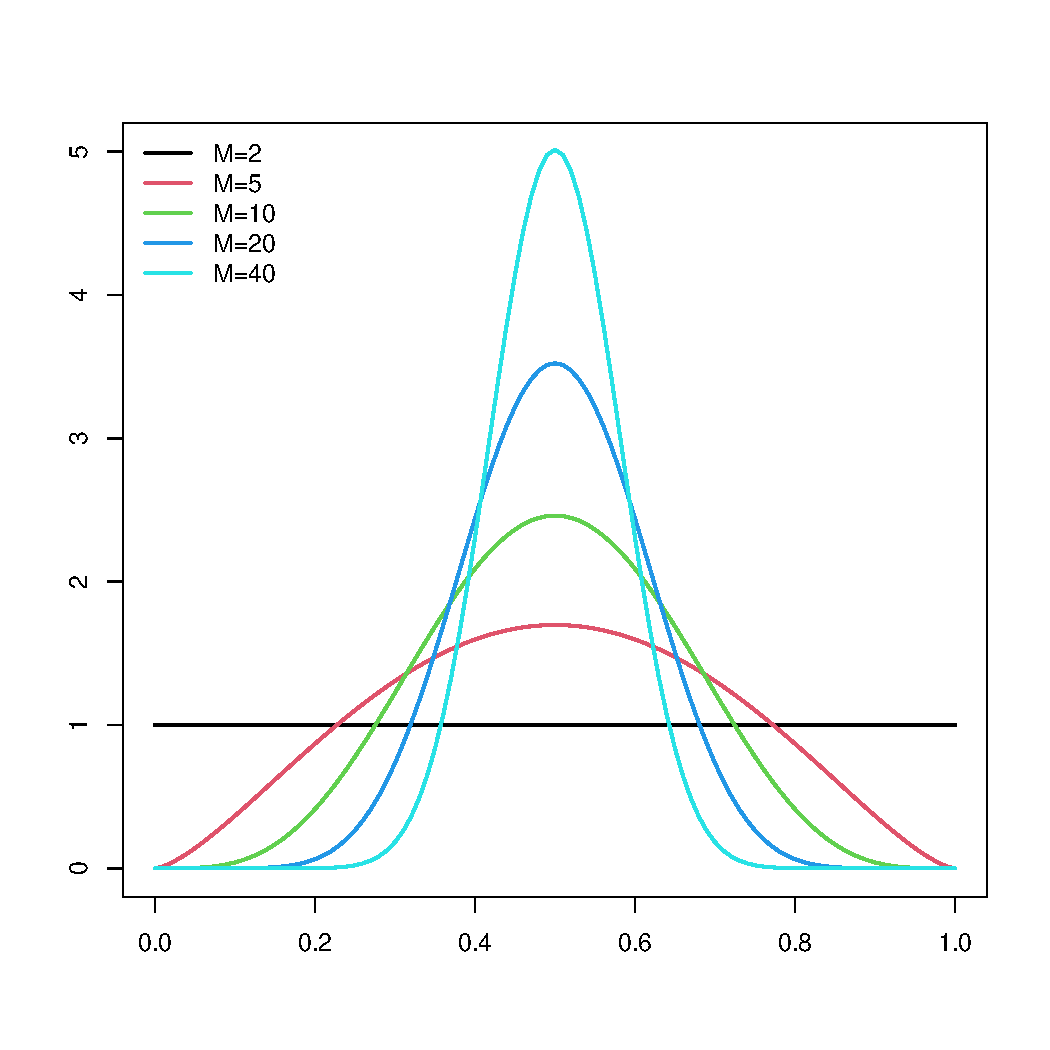
\includegraphics[scale=0.38]{BetaProp_dist.pdf}}]
	{Probabilistic (causal) model}
	{Express variability in BetaProp}
	
	\begin{equ}
		%
		\begin{aligned} 
			%
			H^{O}_{ik} & \sim \; BetaProp( H^{T}_{i}, \textcolor{blue}{ M_{ik} } ) \\
			%
			H^{T}_{i} & = \; \alpha / ( \alpha + \beta ) \\
			%
			M_{ik} & = \; \alpha + \beta \\ \\
			%
			\alpha & = \; H^{T}_{i} \cdot M_{ik} \\
			%
			\beta & = \; (1 - H^{T}_{i} ) \cdot M_{ik} \\ \\
			%
			\alpha & = \; 0.5 \cdot 2 \\
			%
			\beta & = \; (1 - 0.5 ) \cdot 2
			%
		\end{aligned}
		%
		%\caption*{(a) general probabilistic model}
	\end{equ}
	%
\end{lhframe}
%
%
\begin{frame}
	{Interested in two effects}
	%
	\begin{columns}
		%
		\begin{column}{0.5\textwidth}
			%
			\begin{enumerate}
				%
				\item \textcolor{blue}{total effects} model inherits:
				%
				\begin{itemize}
					%
					\item children’s characteristics that lead to the fitting of specific apparatus,
					%
					\item the (convenience of) sample selection \textcolor{blue}{(fixed with post-stratification)}
					%
				\end{itemize}
				%
				\item to do the last, we stratify for all variables that explain variability, ergo, use a \textcolor{blue}{direct effects} model
				%
				\item two levels: replicates ($k$), children ($i$), denoted by discontinuous squares
				%
			\end{enumerate}
			%
		\end{column}
		%
		\begin{column}{0.5\textwidth}  
			%
			\begin{figure}
				%
				\begin{tikzpicture}
					% nodes
					\node at (3,0) {$H^{O}_{ik}$};
					\node at (2,-0.7) {$U_{ik}$};
					\node at (1,-0.4) {$H^{T}_{i}$};
					\node at (-0.5,-0.4) {$SI_{i}$};
					\node at (-1.5,-0.7) {$U_{i}$};
					\node at (-0.9,1.2) {$HS_{i}$};
					%\node at (-0.5,2.7) {$U_{HS}$};
					\node at (-2.2,1) {$E_{i}$};
					%\node at (-2,2.7) {$U_{E}$};
					%\node at (1.5,1.5) {$PTA_{i}$};
					%\node at (1,2.7) {$U_{P}$};
					%\node at (-2,1) {$A_{i}$};
					%\node at (-2.8,1) {$U_{A}$};
					
					% paths
					\draw[{Circle[open]}-{latex}](0.85,0)--(2.6,0); % Hi->Hik
					\draw[{Circle[open]}-{latex}{Circle}](1.9,-0.4)--(2.7,0); % Uik->Hik
					\draw[{Circle[open]}-{latex}](-0.5,0)--(0.85,0); % SIi->Hi
					\draw[{Circle[open]}-{latex}](-1.6,-0.4)--(-0.5,0); % Ui->SIi
					\draw[{Circle}-{latex}](-0.45,1.05)--(-0.45,0.05); % HSi->SIi
					%\draw[-{latex}](-0.45,0.95)--(-1.90,0.75); % HSi->Ai
					\draw[{Circle}-{latex}](-2,1)--(-0.5,1); % Ei->HSi
					\draw[-{latex}](-1.9,1)--(-0.47,0.05); % Ei->SIi
					%\draw[{Circle}-{latex}](1,1.5)--(-0.4,1.5); % PTAi->HSi
					%\draw[-{latex}](0.9,1.45)--(-0.4,0.05); % PTAi->SIi
					%\draw[{Circle}-{latex}](-2,0.75)--(-0.5,0); % Ai->SIi
					%\draw[{Circle[open]}-{latex}](-1.95,2.5)--(-1.95,1.6); % UE->Ei
					%\draw[{Circle[open]}-{latex}](-0.45,2.5)--(-0.45,1.6); % UHS->HSi
					%\draw[{Circle[open]}-{latex}](0.95,2.5)--(0.95,1.6); % UP->PTAi
					%\draw[{Circle[open]}-{latex}](-2.8,0.70)--(-2,0.70); % UA->Ai
					
					% extras
					\node at (0.2,-0.25) {$(-)$}; % symbol
					\draw[dotted, thick] (1.5,0.5) rectangle (3.5,-1);
					%\node at (2,0.7) {$k=1,\dots,K$};
					\draw[dashed] (-2.5,1.45) rectangle (3.7,-1.2);
					%\node at (2,0.7) {$k=1,\dots,K$};
				\end{tikzpicture}
				\caption*{(b) total effects}
			\end{figure}
			%
			\begin{figure}
				%
				\begin{tikzpicture}
					% nodes
					\node at (3,0) {$H^{O}_{ik}$};
					\node at (2,-0.7) {$U_{ik}$};
					\node at (1,-0.4) {$H^{T}_{i}$};
					\node at (-0.5,-0.4) {$SI_{i}$};
					\node at (-1.5,-0.7) {$U_{i}$};
					\node at (-0.9,1.75) {$HS_{i}$};
					%\node at (-0.5,2.7) {$U_{HS}$};
					\node at (-2.2,1.5) {$E_{i}$};
					%\node at (-2,2.7) {$U_{E}$};
					\node at (1.5,1.5) {$PTA_{i}$};
					%\node at (1,2.7) {$U_{P}$};
					\node at (-2.1,1) {$A_{i}$};
					%\node at (-2.8,1) {$U_{A}$};
					
					% paths
					\draw[{Circle[open]}-{latex}](0.85,0)--(2.6,0); % Hi->Hik
					\draw[{Circle[open]}-{latex}{Circle}](1.9,-0.4)--(2.7,0); % Uik->Hik
					\draw[{Circle[open]}-{latex}](-0.5,0)--(0.85,0); % SIi->Hi
					\draw[{Circle[open]}-{latex}](-1.6,-0.4)--(-0.5,0); % Ui->SIi
					\draw[{Circle}-{latex}](-0.45,1.6)--(-0.45,0.05); % HSi->SIi
					\draw[-{latex}](-0.45,1.50)--(-1.90,0.75); % HSi->Ai
					\draw[-{latex}](-0.45,1.5)--(0.9,1.5); % HSi->PTAi
					\draw[{Circle}-{latex}](-2,1.5)--(-0.5,1.5); % Ei->HSi
					\draw[-{latex}](-1.9,1.45)--(-0.47,0.05); % Ei->SIi
					\draw[{Circle[color=red]}-{latex}](0.95,1.55)--(-0.4,0.05); % PTAi->SIi
					\draw[{Circle[color=red]}-{latex}](-2,0.75)--(-0.5,0); % Ai->SIi
					%\draw[{Circle[open]}-{latex}](-1.95,2.5)--(-1.95,1.6); % UE->Ei
					%\draw[{Circle[open]}-{latex}](-0.45,2.5)--(-0.45,1.6); % UHS->HSi
					%\draw[{Circle[open]}-{latex}](0.95,2.5)--(0.95,1.6); % UP->PTAi
					%\draw[{Circle[open]}-{latex}](-2.8,0.70)--(-2,0.70); % UA->Ai
					
					% extras
					\node at (0.2,-0.25) {$(-)$}; % symbol
					\draw[dotted, thick] (1.5,0.5) rectangle (3.5,-1);
					%\node at (2,0.7) {$k=1,\dots,K$};
					\draw[dashed] (-2.5,2) rectangle (3.7,-1.2);
					%\node at (2,0.7) {$k=1,\dots,K$};
				\end{tikzpicture}
				\caption*{(a) direct effects}
			\end{figure}
			%
		\end{column}
		%
	\end{columns}
	%
\end{frame}
%
%
\begin{frame}
	{Probabilistic (causal) model}
	{Second form}
	%
	\begin{columns}
		%
		\begin{column}{0.5\textwidth}
			%
			\begin{equ}
				%
				\begin{aligned} 
					H^{O}_{ik} \leftarrow & \; f(H^{T}_{i}, U_{ik}) \\
					%
					H^{T}_{i} \leftarrow & \; f(SI_{i}) \\
					%
					SI_{i} \leftarrow & \; f(HS_{i}, E_{i}, \textcolor{red}{A_{i}}, \textcolor{red}{PTA_{i}}, U_{i} ) \\ \\ \\
					%
					HS_{i} \leftarrow & \; f(U_{HS}) \\
					%
					A_{i} \leftarrow & \; f(U_{A}) \\
					%
					E_{i} \leftarrow & \; f(U_{E}) \\
					%
					PTA_{i} \leftarrow & \; f(U_{P}) \\
					%
					U \sim & \; P(\pmb{U})
					%
				\end{aligned}
				%
				\caption*{(a) general structural model}
			\end{equ}
			%
		\end{column}
		%
		\begin{column}{0.5\textwidth}  
			%
			\begin{equ}
				%
				\begin{aligned} 
					%
					H^{O}_{ik} & \sim \; BetaProp( H^{T}_{i}, M_{ik}) \\
					%
					H^{T}_{i} & = \; \text{inv\_logit}( -SI_{i} ) \\
					%
					SI_{i} & = \; a_{i} + \alpha + \alpha_{E[i],HS[i]} + \textcolor{red}{\beta_{P} PTA_{i}} \\ 
					%
					& \quad + \textcolor{red}{\beta_{A, HS[i]} (A_{i} - \bar{A})} \\
					%
					a_{i} & \sim \; Normal( 0, \sigma_{Ui}) \\
					%
					HS_{i} & \sim \; \text{data} \\
					%
					A_{i} & \sim \; \text{data} \\
					%
					E_{i} & \sim \; \text{data} \\
					%
					PTA_{i} & \sim \; \text{data} \\
					%
					U & \sim \; \text{unobservable}
					%
				\end{aligned}
				%
				\caption*{(a) general probabilistic model}
			\end{equ}
			%
		\end{column}
		%
	\end{columns}
	%
\end{frame}
%
%